%-------------------------
%minimal-unix
%(c) H.Buchmann FHNW 2014
%export TEXINPUTS=.:${HOME}/fhnw/edu/:${HOME}/fhnw/edu/tinL/config/latex:${HOME}/fhnw/edu/config//:
%-------------------------
\documentclass{beamer}
\usepackage{latex/beamer}
%---------------------
%local defines
%(c) H.Buchmann FHNW 2009
%$Id$
%---------------------
\newcommand{\target} {\beaglebone\xspace}
\newcommand{\targetS}{{\bf BBG}\xspace}
\newcommand{\host}   {{\em Host}\xspace}
\newcommand{\targetroot} {{\bf target-root}\xspace}
\newcommand{\kernel} {{\bf kernel}\xspace}
\renewcommand{\c}{{\bf C}\xspace}
\newcommand{\cpp}{{\bf C++}\xspace}
\newcommand{\posix}{{\bf POSIX}\xspace}

\input{/home/buchmann/latex/dirtree/dirtree.tex}

\usepackage[absolute]{textpos}
\setlength{\TPHorizModule}{1mm}
\setlength{\TPVertModule}{1mm}

\begin{document}


\title[udev]{udev\\die Verwaltung von Devices}

\frame{\titlepage}

\begin{frame}{The Big Picture}{Hardware calls Software}
 \begin{itemize}
  \item {\em Devices} k�nnen zu einer beliebigen Zeit 
  \begin{itemize}
   \item angeschlossen
   \item entfernt
  \end{itemize}
  werden
  \item zu einem {\em Device} geh�rt ein {\em Driver}
 \end{itemize}
\end{frame}

\begin{frame}[fragile]{Typisches Beispiel}{USB {\em Device}}
 \begin{enumerate}
  \item USB {\em Device} einstecken
  \item Betriebssystem muss den richtigen {\em Driver}
  \begin{itemize}
   \item finden
   \item konfigurieren
  \end{itemize}
 \end{enumerate}
 \begin{block}{Das tool}
 \begin{lstlisting}[language=bash]
 udevadm monitor
 \end{lstlisting}
 \end{block}
\end{frame}

\begin{frame}{Hardware calls Software}{call back}
\begin{center}
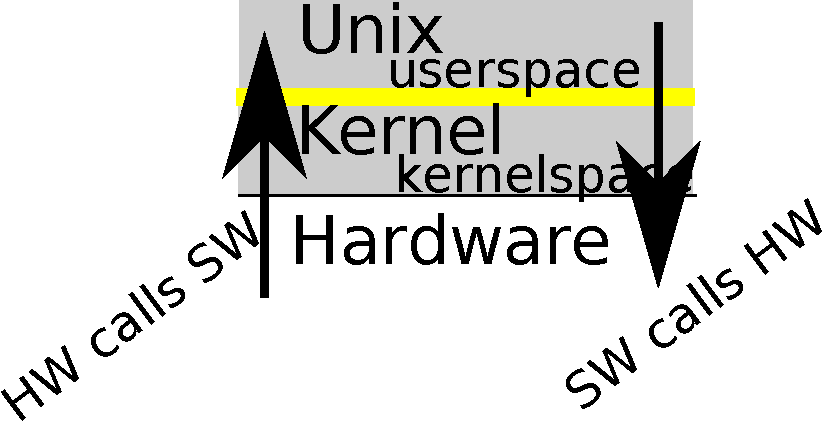
\includegraphics[width=0.875\textwidth]{hw-calls-sw.pdf}
\end{center}
\end{frame}

\begin{frame}{Hardware calls Software}{call back}
 \begin{enumerate}
  \item {\em Hardware} registriert �nderung: {\em Interrupt}
  \begin{itemize}
   \item USB {\em Device} eingesteckt
  \end{itemize}
  \item {\em Kernel} informiert \unix
  \begin{itemize}
   \item USB type etc.
  \end{itemize}
  \item \unix installiert/konfiguriert {\em Driver}  
 \end{enumerate}
\end{frame}

\section{udev}

\begin{frame}{udev:Dynamic device management}{userspace}
 \begin{block}{Rule}
  \begin{itemize}
   \item beschreibt was f�r ein oder meherer Ger�te zu tun ist
   \item Siehe \cod{man udev}, \cod{man udevadm}
  \end{itemize}
 \end{block}
\end{frame}

\begin{frame}{Aufgabe}{SD-Card richtig montieren}
 \begin{itemize}
  \item \cod{udevadm monitor}
  \item \cod{udevadm test}
  \item \cod{udevadm control -R} reload
  \item eigene {\em rule} in \cod{/etc/udev/rules.d}
  \begin{itemize}
   \item \cod{RUN} eigenes Programm
  \end{itemize}
 \end{itemize}
\end{frame}

\end{document}
